\documentclass{beamer}
\graphicspath{{./images/}}
\renewcommand\L{\mathcal{ L}}
\renewcommand{\epsilon}{\varepsilon}
\renewcommand{\div}[1]{\operatorname{div}\left( #1 \right)}

\usetheme{Warsaw}
\usecolortheme{beaver}
\title[Numerical homogenization]{Numerical Homogenization in Fenics}
%\subtitle{An exploration}
\author[O. Richardson \and I. Stefansson] % (optional, for multiple authors)
{Omar Richardson \and Ivar Stefansson}
\institute % (optional)
{
    Karlstad University, Sweden \and University of Bergen, Norway
}
\date[]{Nordic Computational Course, 2017}
\subject{Numerical Homogenization 1}

\begin{document}
  \frame{\titlepage}
\begin{frame}{Homogenisation}
    \begin{columns}
        \begin{column}[c]{.5\textwidth}
            Simulation of flow through nonhomogeneous (material)
            \begin{itemize}
              \item Conduction through composite materials
              \item Ground water flow
            \end{itemize}
        \end{column}
        \begin{column}[c]{.5\textwidth}
            .
        \end{column}
    \end{columns}
\end{frame}

\begin{frame}[t]{Project aim}
    \begin{itemize}
        \item Get aquainted with homogenization theory
        \item Implement automated upscaled solution solving in Fenics
        \item Experiment with different solvers and preconditioners
    \end{itemize}
\end{frame}

\begin{frame}[t]{Model}
    Let $\varepsilon>0$. Find $u(x)$ s.t.
    \begin{equation}
        \begin{split}
            -\div{A_\varepsilon(x)\nabla u(x))} &= f(x) \mbox{ for } x \in \Omega,\\
            u_\varepsilon(x) &= 0 \mbox{ for } x \in \partial\Omega.
        \end{split}
        \label{eq:model}
    \end{equation}
     $A_\varepsilon(x)$ has period $\varepsilon$.

\end{frame}

\begin{frame}[t]{Upscaling}
    Scale separation: \begin{itemize}
        \item Macroscopic $x$, microscopic $y:= x/\varepsilon$.
        \item Ansatz: power expansion: $u_\varepsilon(x,y) = \sum_i \varepsilon^i u_i(x,y)$
        \item $\nabla u_i(x) = \varepsilon^{-1}\nabla_yu_i + \nabla_xu_i(x,y)$
    \end{itemize}
    .\\
    then we obtain $\lim_{\varepsilon\to 0} u_\varepsilon = u_0$
\end{frame}

\begin{frame}[t]{Weak Form}
    For all $\phi \in H^1_0(Y)$
    \begin{equation}
        A(y)\nabla w_i \nabla \phi = \div{(A(y)e_i)}\phi
        \label{eq:weak_cell_problem}
    \end{equation}
\end{frame}

\begin{frame}[t]{Exact solution (1D)}
    Let \begin{itemize}
        \item $\Omega = [0,1]$
        \item $f(x) = 1$
        \item $A_\varepsilon(x) = \left( 2+\cos\left(\frac{2\pi x}{\epsilon}\right) \right)^{-1}$
    \end{itemize}
    then $u_\varepsilon(x)$ is a (strong) solution:
    \[ u(x) = \left( \frac{1}{2} - x \right) \left(2x + \frac{\epsilon}{2\pi}\sin\left(\frac{2\pi x}{\epsilon}\right) \right) + \frac{\epsilon^2}{(2\pi)^2}\left( 1 - \cos \left( \frac{2\pi x}{\epsilon} \right) \right) + x^2 \]
\end{frame}

\begin{frame}[t]{Numerical/Upscaled solution}

\end{frame}

\begin{frame}[t]{Convergence rates}

\end{frame}

\begin{frame}[t]{2D approximation}
  \begin{columns}
    \begin{column}[c]{.6\textwidth}
      \begin{itemize}
        \item
        %\begin{equation}
         $ A_\epsilon(x) =  \left( 2+\cos\left(\frac{2\pi(x+2y)}{\epsilon}\right) \right)^{-1}$
        %\end{equation}
       \item Solve cell problem with relatively high resolution.
       \item Remaining error:
      \begin{itemize}
        \item Model, $\epsilon > 0$
        \item Finite solution of the global problem, $h_{global} > 0$
        \item Convergence in both $\epsilon$ and $h_{global}$.
       \end{itemize}
      \end{itemize}
    \end{column}
    \begin{column}[c]{.4\textwidth}
      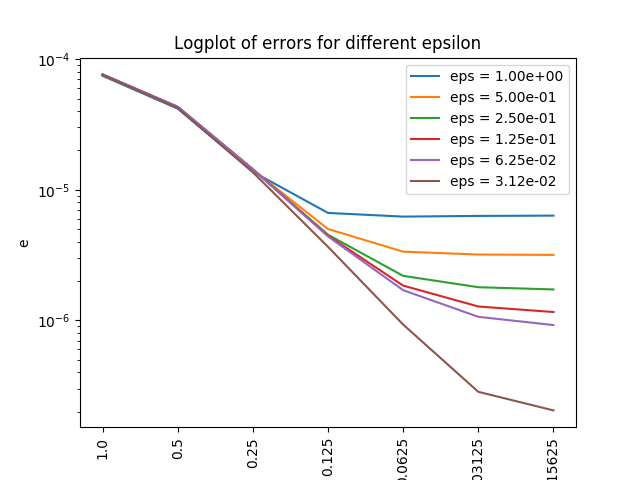
\includegraphics[width=0.9\linewidth]{2d_global_errors.png}      % 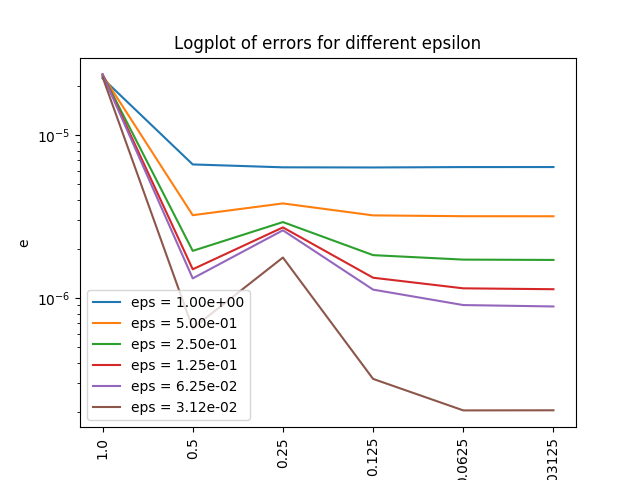
\includegraphics[width=0.65\linewidth]{2d_cell_errors.png}
    \end{column}
  \end{columns}

\end{frame}

\begin{frame}[t]{Solvers \& preconditioners}
  \begin{columns}
    \begin{column}[c]{.5\textwidth}
      \begin{itemize}
      \item Incomplete LU and Conjugate Gradient good for symmetric problems.
      \item GMRES expensive, convergence not granted for increased number of cells.
    \end{itemize}
  \end{column}
  \begin{column}[c]{.5\textwidth}

    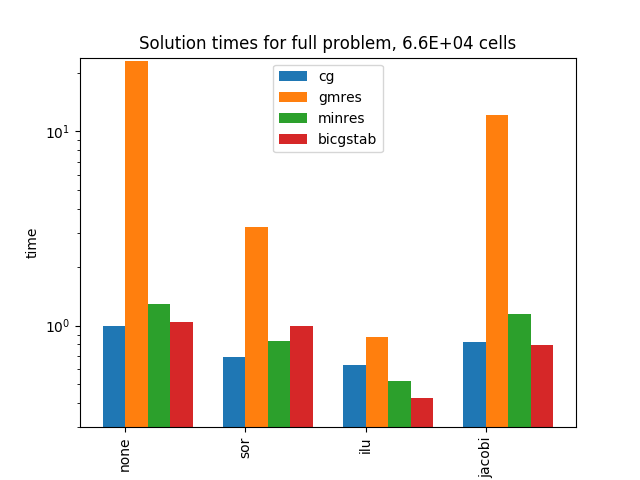
\includegraphics[width=0.9\linewidth]{SolverTimesFullh8.png}

    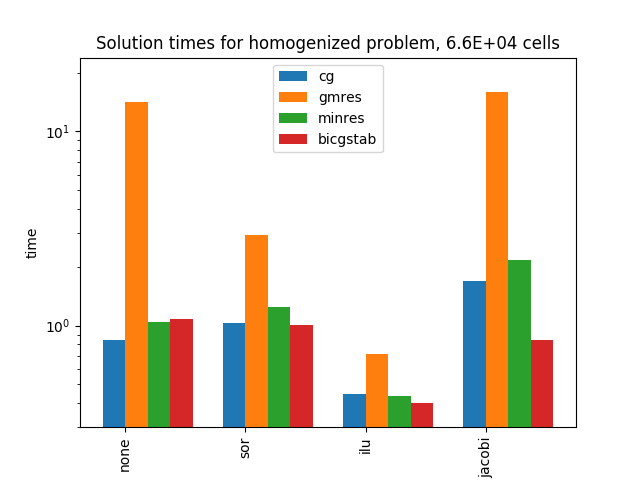
\includegraphics[width=0.9\linewidth]{SolverTimesHomoh8.png}

 \end{column}
\end{columns}
\end{frame}

\begin{frame}[t]{Application I}
  \begin{columns}
    \begin{column}[c]{.5\textwidth}
      \begin{itemize}
      \item Resolution of small $\epsilon$ unachievable due to complexity.
      \item Convergence in the  $\epsilon$ limit.
      \end{itemize}
      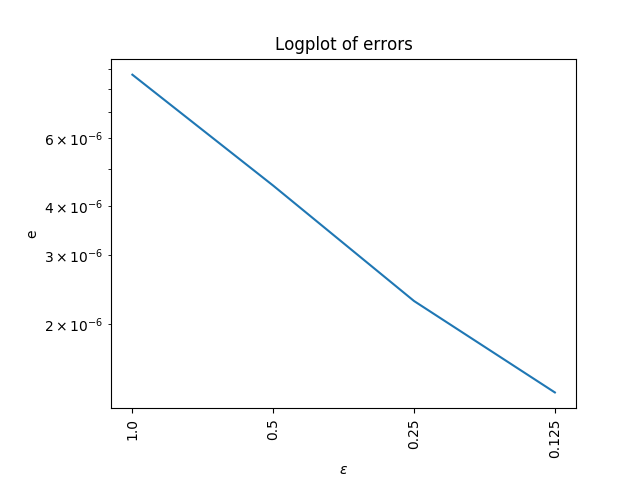
\includegraphics[width=0.65\linewidth]{carw_errors.png}
  \end{column}
  \begin{column}[c]{.5\textwidth}

    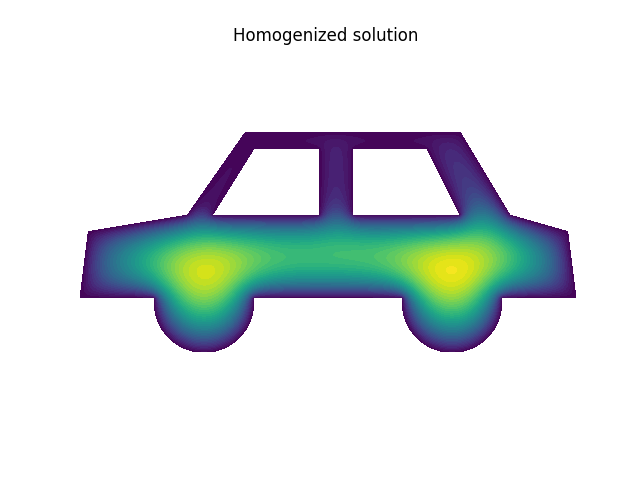
\includegraphics[width=0.65\linewidth]{carw_homogenized.png}

    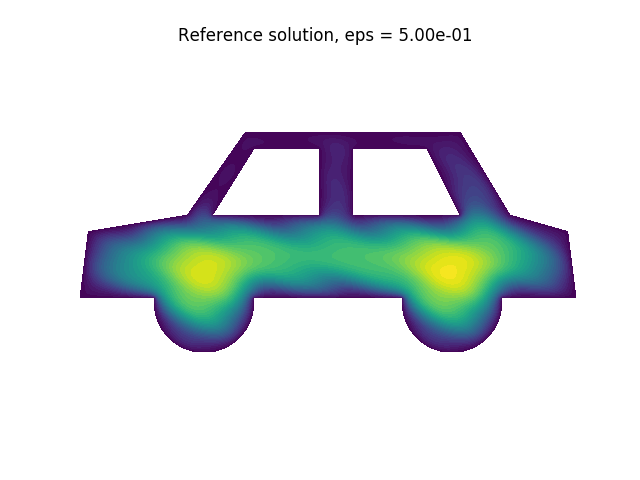
\includegraphics[width=0.65\linewidth]{carw_reference_eps_power_1.png}

    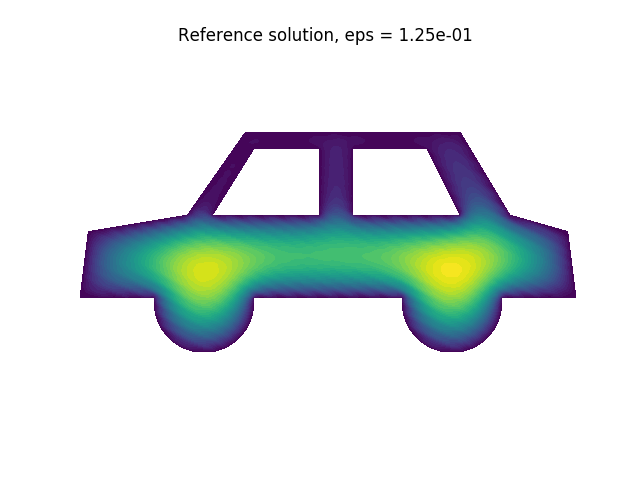
\includegraphics[width=0.65\linewidth]{carw_reference_eps_power_3.png}

 \end{column}
\end{columns}
\end{frame}

\begin{frame}[t]{Application II}
  \begin{columns}
    \begin{column}[c]{.5\textwidth}
      \begin{itemize}
      \item Three dimensions and time dependency add to computational cost.
      \item Homogenization usually only possibility, allows for simulations on a range of different applications.
    \end{itemize}
  \end{column}
  \begin{column}[c]{.5\textwidth}

 \end{column}
\end{columns}

\end{frame}
\end{document}
